\documentclass[10pt]{mypackage}

% sans serif font:
%\usepackage{cmbright}
%\usepackage{sfmath}
%\usepackage{bbold} %better blackboard bold

%serif font + different blackboard bold for serif font
\usepackage{newpxtext,eulerpx}
\renewcommand*{\mathbb}[1]{\varmathbb{#1}}
\renewcommand*{\hbar}{\hslash}

\pagestyle{fancy} %better headers
\fancyhf{}
\rhead{Avinash Iyer}
\lhead{Physics 310: Assignment 4}

\setcounter{secnumdepth}{0}

\begin{document}
\RaggedRight
\section{Chapter 11 Problems}%
\subsection{Problem 1}%
\begin{enumerate}[(a)]
  \item $\mathbf{F}\left(\mathbf{x}\right) = \frac{1}{\rho}\hat{\rho}$.
    \begin{center}
      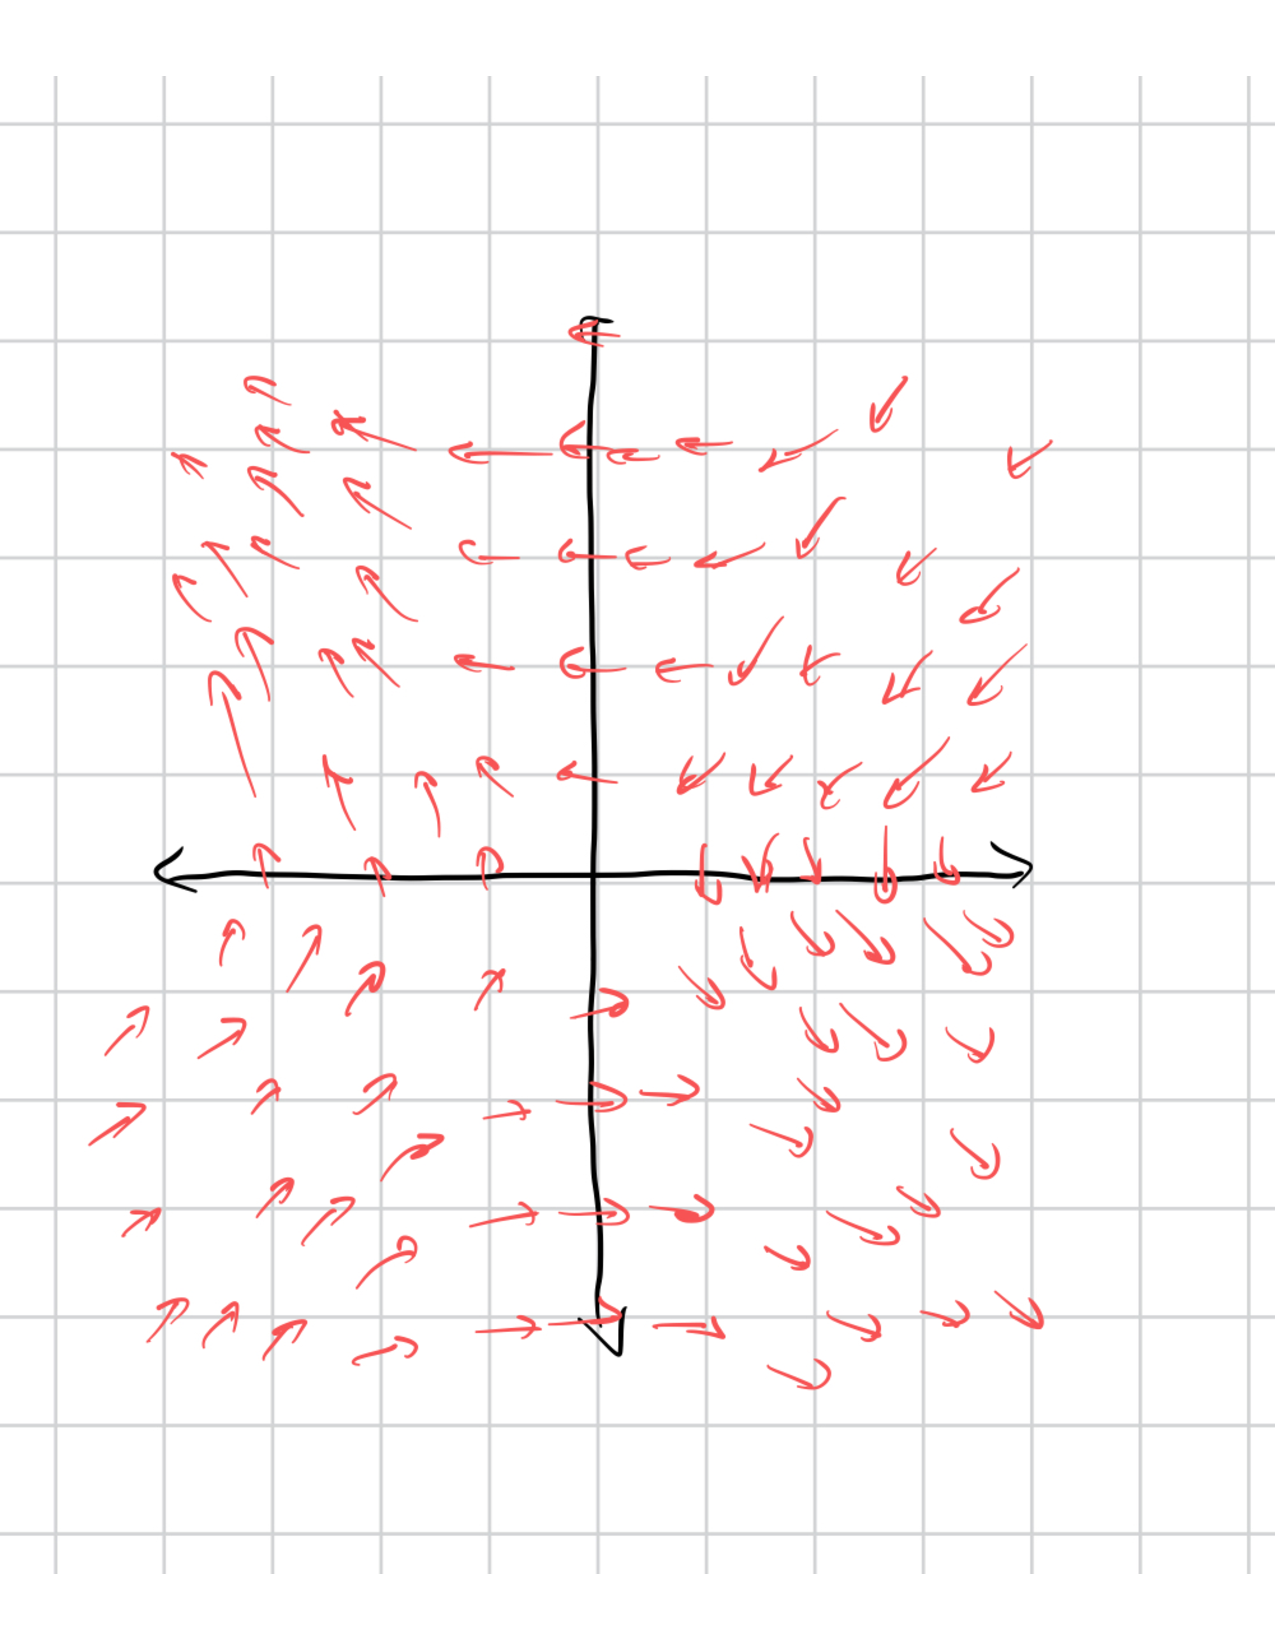
\includegraphics[width=10cm]{images/p_2a_1_11-1a.pdf}
    \end{center}
  \item $\mathbf{F}\left(\mathbf{x}\right) = y\hat{i} + x\hat{j}$.
    \begin{center}
      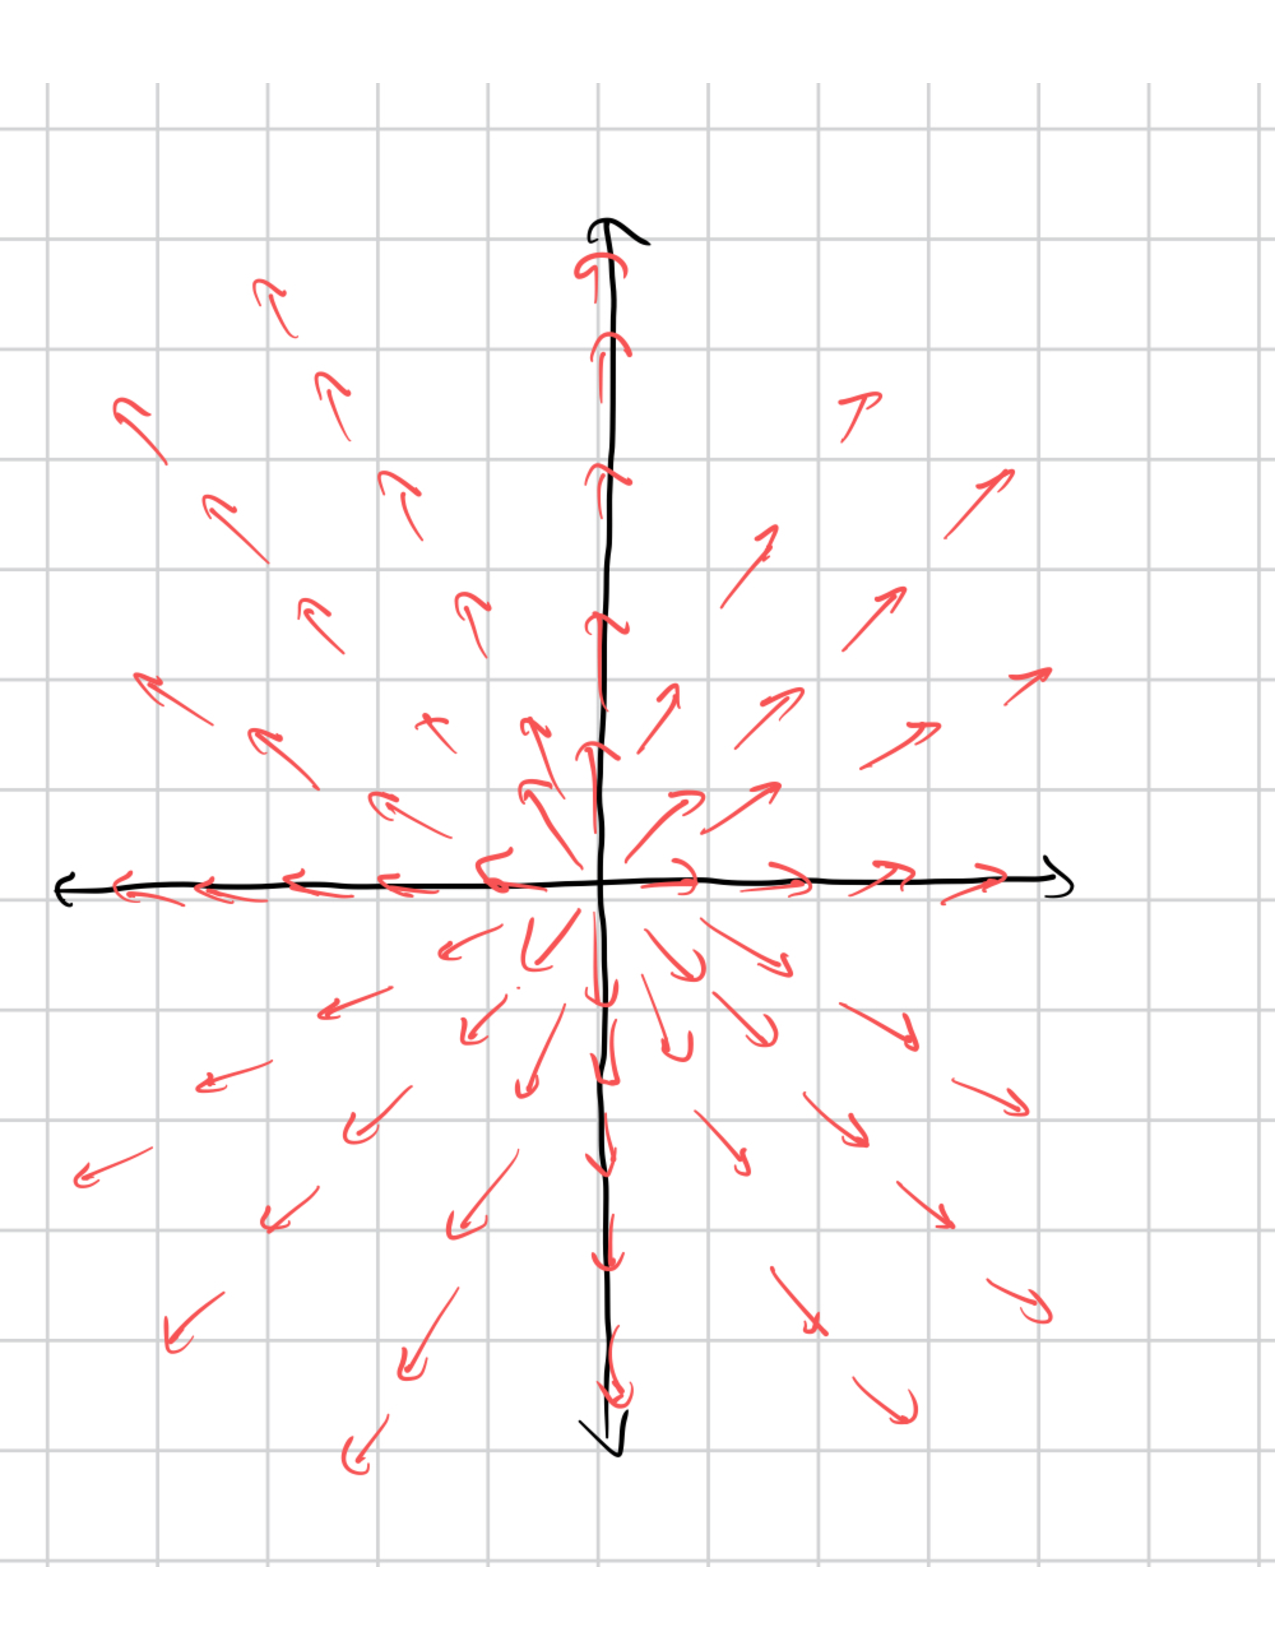
\includegraphics[width=10cm]{images/p_2a_1_11-1b.pdf}
    \end{center}
\end{enumerate}
\subsection{Problem 2}%
The parametrized streamlines for $\mathbf{v} = \left(-y,x\right)$ are of the form $r\cos t \hat{i} + r\sin t \hat{j}$.
\subsection{Problem 3}%
We can see that $\mathbf{E}$ and $\mathbf{B}$ are mutually perpendicular by taking the standard inner product
\begin{align*}
  \iprod{xy^2\hat{i} + x^2y\hat{j}}{x^2y\hat{i} - xy^2\hat{j}} &=0.
\end{align*}
Additionally, for $\mathbf{E}$,
\begin{align*}
  \diff{y}{t} &= x^2 y\\
  \diff{x}{t} &= xy^2\\
  \diff{y}{x} &= \frac{x}{y}\\
  y^2 &= x^2 + K,
\end{align*}
and for $\mathbf{B}$,
\begin{align*}
  \diff{y}{t} &= -xy^2\\
  \diff{x}{t} &= x^2 y\\
  \diff{y}{x} &= -\frac{y}{x}\\
  y &= \frac{K}{x}.
\end{align*}
\subsection{Problem 4}%
\begin{enumerate}[(a)]
  \item 
    \begin{align*}
      \int_{V}^{} \mathbf{E}\left(\mathbf{r}\right)\:d^3x &= \int_{0}^{\pi/2}\int_{0}^{2\pi}\int_{0}^{R} \hat{r}\sin\theta \:drd\phi d\theta\\
      \int_{V}^{} \mathbf{E}\left(\mathbf{r}\right)\:d^3 x &= \int_{-R}^{R}\int_{-\sqrt{R^2-x^2}}^{\sqrt{R^2-x^2}}\int_{0}^{\sqrt{R^2-x^2 - y^2}} \frac{x\hat{i} + y\hat{j} + z\hat{k}}{\left(x^2 + y^2 + z^2\right)^{3/2}}\:dz dy dx
    \end{align*}
  \item 
    \begin{align*}
      \int_{V}^{} \mathbf{E}\left(\mathbf{r}\right)\:d^3 x &= \int_{0}^{\pi/2}\int_{0}^{2\pi}\int_{0}^{R} \sin\theta \left(\cos\phi\sin\theta\hat{i} + \sin\phi\sin\theta\hat{j} + \cos\theta\hat{k}\right)\:dr d\phi d\theta
    \end{align*}
    This integral is more practical than the pure forms since the basis is position-independent and the integral is not a giant mess.
  \item Using symmetry, since $\cos\phi$ is integrated from $0$ to $2\pi$ and $\sin\phi$ is integrated from $0$ to $2\pi$, both the $\hat{i}$ and $\hat{j}$ components are $0$.
    \begin{align*}
      \int_{0}^{\pi/2} \sin^2\theta \int_{0}^{2\pi}\cos\phi\int_{0}^{R}\:dr d\phi d\phi &= 0\\
      \int_{0}^{\pi/2} \sin^2\theta \int_{0}^{2\pi}\sin\phi\int_{0}^{R}\:dr d\phi d\phi &= 0
    \end{align*}
  \item Evaluating the $\hat{k}$ component,
    \begin{align*}
      \int_{0}^{\pi/2}\sin\theta\cos\theta \int_{0}^{2\pi}\int_{0}^{R} \:dr d\phi d\theta &= 2\pi R \int_{0}^{\pi/2} \sin\theta\cos\theta\:d\theta\\
                                                                                          &= \pi R.
    \end{align*}
\end{enumerate}
\subsection{Problem 5}%
\begin{align*}
  \mathbf{R}_{\text{cm}} &= \frac{1}{M}\int_{S}^{} \mathbf{r}\:dm\\
                         &= \frac{\sigma}{M}\int_{-\ell/2}^{\ell/2}\int_{0}^{\pi} \left(R\cos\phi\hat{i} + R\sin\phi\hat{j} + z\hat{k} \right)R\:d\phi dz\\
                         &= \frac{\sigma}{M} \left(2R^2\right) \hat{j}.
\end{align*}
\section{Chapter 12 Problems}%
\subsection{Problem 1}%
\subsection{Problem 2}%
\subsection{Problem 3}%
\subsection{Problem 6}%
\subsection{Problem 7}%
\subsection{Problem 9}%
\subsection{Problem 15}%
\subsection{Problem 19}%

\section{Chapter 13 Problems}%
\subsection{Problem 2}%

\end{document}
